\documentclass[11pt]{article}

\usepackage[a4paper,margin=1in]{geometry}
\usepackage[T1]{fontenc}
\usepackage[utf8]{inputenc}
\usepackage{lmodern}
\usepackage{setspace}
\usepackage{amsmath,amssymb}
\usepackage{booktabs}
\usepackage{siunitx}
\usepackage{hyperref}
\usepackage{graphicx}
\usepackage{xcolor}

\hypersetup{
  colorlinks=true,
  linkcolor=blue!50!black,
  citecolor=blue!50!black,
  urlcolor=blue!50!black
}

\title{\textbf{Supplementary Information}\\
for\\
\textbf{Learning Spatially Heterogeneous Copulas from Marginal Constraints\\
via Distribution-Level Diffusion for Population Synthesis}}

\author{Jinlin Wu$^{1}$, Collaborators$^{1}$\\
\small $^{1}$Synthetic City Project}
\date{}

\begin{document}
\maketitle
\onehalfspacing
\renewcommand{\figurename}{Supplementary Fig.}
\renewcommand{\thefigure}{S\arabic{figure}}

\section{Supplementary Methods}
This SI reports implementation details omitted from the main manuscript, including complete condition definitions, binning mappings, and post-hoc IPF settings.

\section{Supplementary Results}

\subsection{Person-level diffusion fails to recover regional dependence}

To verify that training on individual records is insufficient for copula recovery, we ran a separate experiment using person-level conditional diffusion on Michigan household demographics (age $\times$ income, $K=100$ bins) with region identity as an explicit conditioning variable. The model was evaluated using five-fold spatial cross-validation across Michigan's 68 PUMAs. As shown in Supplementary Fig.~\ref{fig:si_person_level}, person-level diffusion produced \emph{worse} copula TVD (mean = 0.159) than a na\"ive baseline that simply reuses the training-set average dependence structure (mean = 0.137). This degradation was consistent across all five folds and affected 75\% of individual PUMAs (51 of 68 above the diagonal in panel b). The result confirms that per-sample training losses do not provide a sufficient learning signal for aggregate dependence recovery.

\begin{figure}[!htb]
\centering
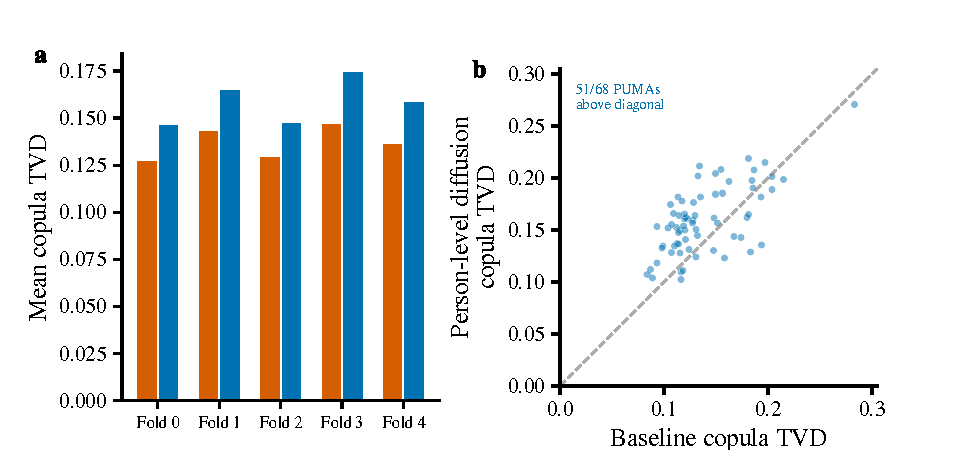
\includegraphics[width=\textwidth]{figures/fig_si_person_level.pdf}
\caption{\textbf{Person-level diffusion fails to recover copula.}
\textbf{(a)}~Five-fold mean copula TVD for person-level conditional diffusion (blue) versus training-set average baseline (orange). The diffusion model is systematically worse in every fold.
\textbf{(b)}~Per-PUMA comparison across all folds. Points above the diagonal indicate PUMAs where diffusion produced worse copula TVD than the baseline; 51 of 68 PUMAs (75\%) fall above the line.}
\label{fig:si_person_level}
\end{figure}

This SI also provides full ablation outputs, training-length sensitivity, and additional robustness diagnostics across all evaluated configurations.

\section{Run Artifact Index}
Key result directories and machine-readable summaries are maintained in the project outputs. For submission, include the finalized artifact table matching the camera-ready manuscript.

\section{Reproducibility Notes}
All scripts for preprocessing, training, and evaluation are in the repository. Figure-generation scripts are kept outside the Overleaf package and used only for local regeneration.

\bibliographystyle{unsrt}
\bibliography{references}

\end{document}
